\documentclass[../main.tex]{subfiles}
\addbibresource{../bibfile.bib}


% Tecnologie da spiegare
% - Ghidra
% - angr
% - Flask (Cenni)
% - SvelteKit (Cenni)

\begin{document}

\chapter{Tecnologie utilizzate}
\label{chap:conclusion}
Questo capitolo è dedicato ad un'analisi dettagliata delle principali tecnologie adottate per lo sviluppo della piattaforma Binoculars.
Verrà approfondito il funzionamento e la struttura interna per ogni tecnologia impiegata e quali funzionalità essa offre nell'ambito dell'analisi di
file binari.
\section{Capstone}
\textit{Capstone} \cite{Capstone_docs} è una framework leggero e multi-piattaforma per effettuare il disassembly di codice macchina.
Si basa sulla famiglia di framework per compilatori \textit{LLVM}, in particolare sul modulo \textit{LLVM-Machine Code} (LLVM-MC), il quale contiene un disassemblatore interno con supporto
per molteplici architetture. Questo supporto è dato dalla presenza di molteplici \textit{tabelle descrittive} (file \textit{.TD}), le quali descrivono in maniera astratta tutte le caratteristiche
dell'ISA di una determinata architettura. 
Capstone sfrutta queste tabelle per estrarre le seguenti \textbf{informazioni semantiche}:
\begin{itemize}
    \item \textbf{Registri impliciti}: I registri letti e/o scritti \textbf{implicitamente dall'istruzione}; questi registri infatti non appaiono esplicitamente nella stringa della operazione.
    \item \textbf{Gruppi di istruzioni}: A quale categoria funzionale (es. aritmetica, logica, ...) appartiene l'istruzione
\end{itemize}
Per ogni istruzione macchina, Capstone produce una struttura dati di output denominata \textit{cs\_insn}, la quale contiene due tipi di informazioni:
\begin{itemize}
    \item \textbf{Informazioni di base (Indipendenti dall'architettura)}: ID, dimensioni (in byte), mnemonic, e una stringa contenete gli operandi dell'istruzione
    \item \textbf{Informazioni dettagliate}: Contiene le informazioni estratte dal file \textit{.TD}
\end{itemize} 
\begin{figure}[H]
    \centering
    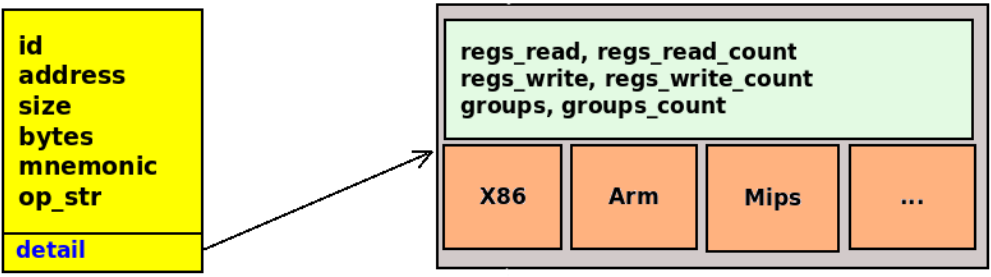
\includegraphics[width = 0.80\textwidth]{../images/cs_isns.png}
    \caption{Struttura interna di cs\_isns. Immagine proveniente da \cite{Capstone_docs}}
\end{figure}
\section{Ghidra}
\textit{Ghidra} è un framework di reverse engineering sviluppato dalla \textit{National Security Agency} degli Stati Uniti d'America \cite{eagle2020ghidra}.
La piattaforma che il framework offre contiene un disassembler, un decompiler e un vasto insieme di tool e script di analisi. Inoltre, la piattaforma può essere
estesa tramite l'aggiunta di plugin e script di analisi personalizzati scritti in python o Java (il linguaggio in cui Ghidra è scritto). In particolare, è possibile interagire con le API messe a disposizione da Ghidra
direttamente da python, utilizzando la libreria \textit{pyghidra}, originariamente sviluppata dal \textit{Department of Defense Cyber Crime Center}(DC3) (un dipartimento del governo americano) e ora parte integrante del progetto Ghidra.
L'architettura di Ghidra è estremamente complessa e formata da diversi moduli software, di cui i principali sono \cite{eagle2020ghidra}:
\begin{itemize}
    \item \textbf{Ghidra loaders}: Questi moduli si occupano dell'importazione dei file binari all'interno della piattaforma. Ogni loader è pensato per un singolo tipo di file eseguibile (ELF, Windows PE, ...). Ghidra permette inoltre di estendere
    l'insieme di loader disponibili tramite l'aggiunta di loader scritti dall'utente stesso.
    \item \textbf{Ghidra processors}: I Ghidra processors sono i moduli più complessi dell'intera piattaforma e si occupano di tutte le operazioni riguardanti il disassembly del file binario. Similmente ai file \textit{.TD} visti per Capstone, anche il processo di disassembly di Ghidra utilizza
    dei file di specifica dell'ISA delle varie architetture supportate. Questi file sono scritti usando il linguaggio specifico per Ghidra denominato \textit{SLEIGH}.
    \item \textbf{Ghidra decompiler}: Questo modulo si occupa del processo di decompilazione del fine binario in una rappresentazione ad alto livello ispirata al linguaggio \textit{C}. Il processo di decompilazione di ghidra avviene in tre fasi distinte:
    \begin{enumerate}
        \item Il decompiler usa i file scritti in SLEIGH per creare una bozza del codice ad alto livello nel linguaggio di rappresentazione intermedia \textit{p-code}. Inoltre, in questa fase viene derivato il CFG del programma
        \item Il codice viene raffinato, eliminando gli statement irraggiungibili o inutili. A seguito di questa operazione, avviene anche una ristrutturazione del CFG in modo da riflettere i potenziali cambiamenti introdotti al flusso di controllo del programma
        \item Viene generato il codice decompilato in un linguaggio \textit{C-like}
    \end{enumerate}
\end{itemize}
\begin{figure}[H]
    \centering
    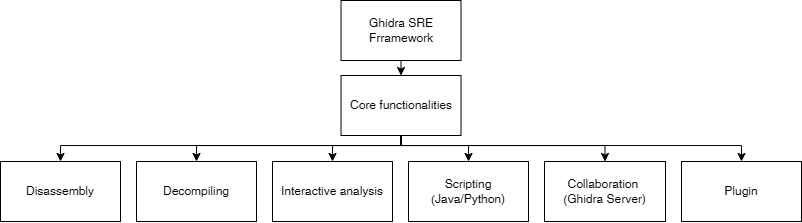
\includegraphics[width = \textwidth]{../images/ghidra.png}
    \caption{Architettura del framework Ghidra}
\end{figure}
\section{angr}










\end{document}